%&pdflatex
\section{Configurazione di rete}
Se il lettore ha seguito il consiglio che avevamo dato nel paragrafo \vref{sec:starting-debian} di attaccare il cavo Ethernet al proprio computer, Debian dovrebbe aver effettuato la configurazione automatica della rete. Se ciò non è successo, è necessario configurarla manualmente seguendo la procedura guidata che non verrà trattata in questo testo.

A questo punto Debian ci chiederà di impostare l'\textit{hostname} della macchina (Figura \vref{fig:hostname-selection}).

\begin{figure}[ht]
	\centering
	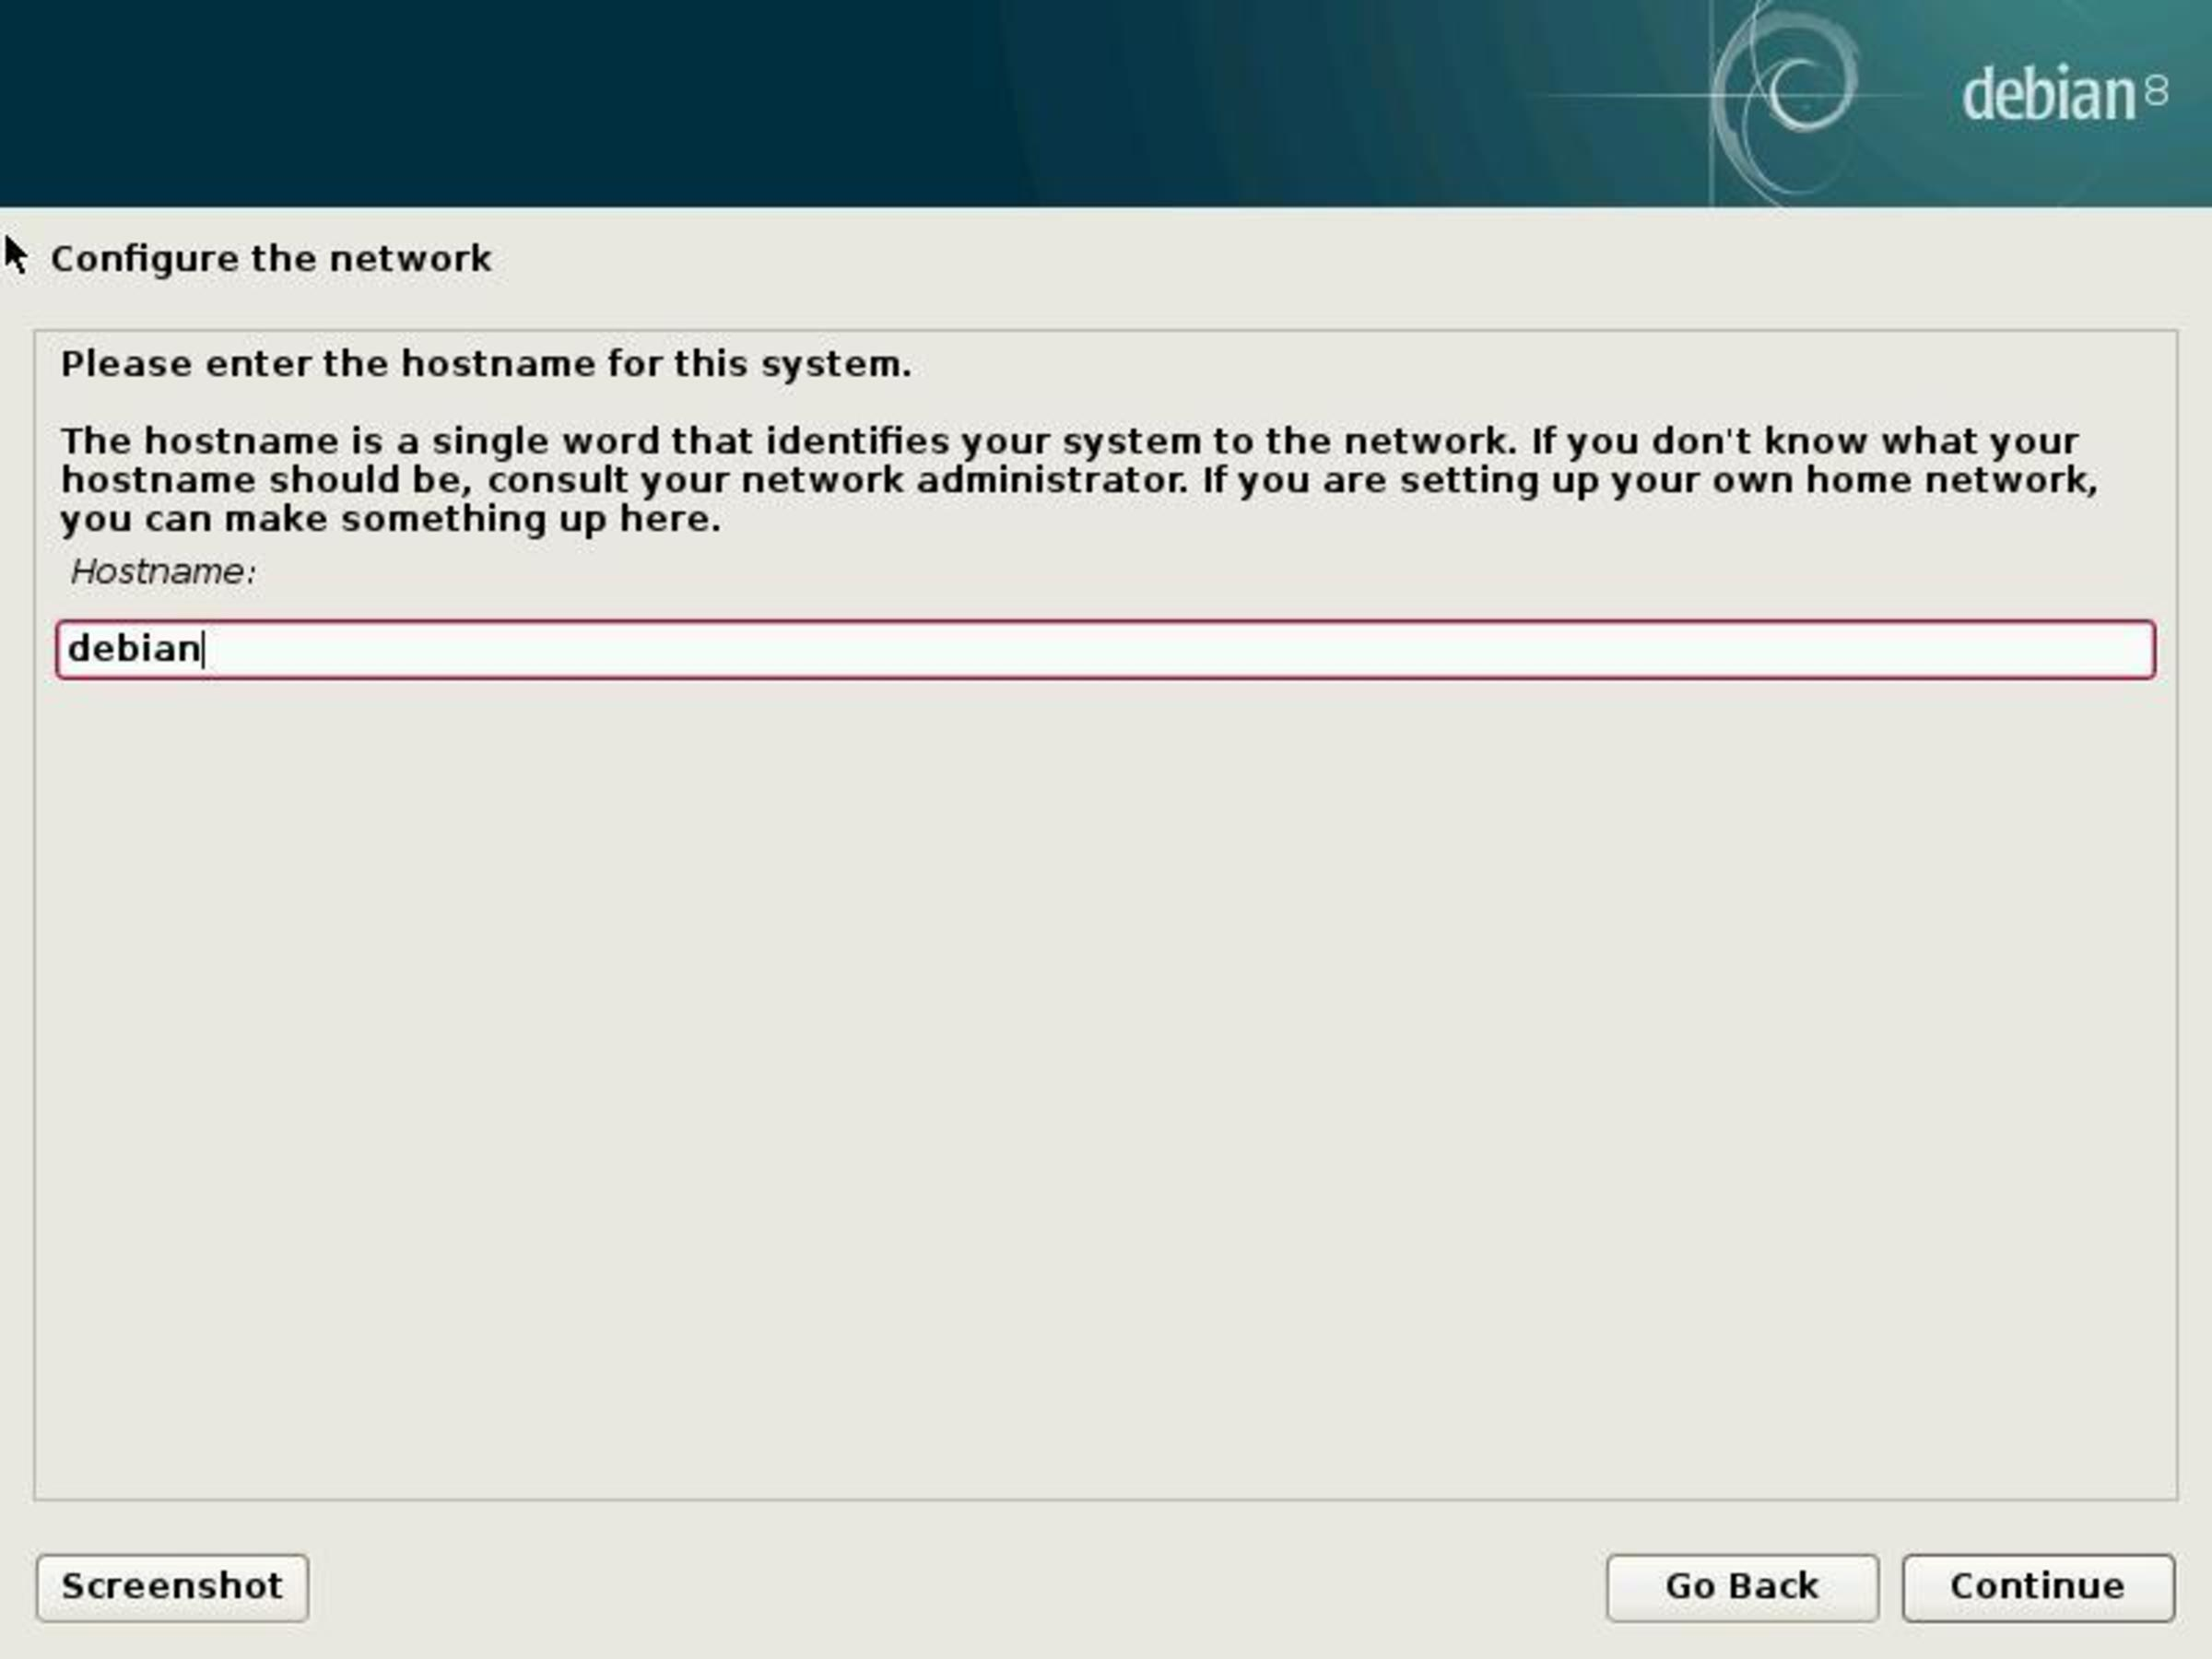
\includegraphics[resolution=600]{hostname-selection}
	\caption{Selezione di un hostname}
	\label{fig:hostname-selection}
\end{figure}

L'hostname è ciò che in Windows viene chiamato \textit{"nome del PC"}. È possibile scegliere qualsiasi cosa come hostname: solitamente, per evitare problemi con alcune applicazioni, si imposta \texttt{localhost} --- ma anche \texttt{debian} va bene, o qualsiasi altra cosa.

Dopodiché, Debian ci chiederà di impostare il dominio da appendere all'hostname. Solitamente questo campo si lascia vuoto, ma anche qui si può scegliere qualsiasi cosa.
